\documentclass{standalone}
\usepackage[T1]{fontenc}
\usepackage[utf8]{inputenc}
\usepackage{pgf,tikz}
\usepackage{pgfplots}
\pgfplotsset{compat=1.9}

\begin{document}

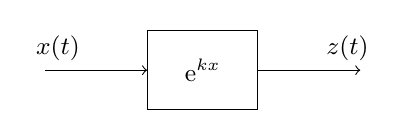
\begin{tikzpicture}[%
  node distance=2cm,
  block/.style={rectangle, draw, minimum width=14mm, minimum height=10mm},]
  {\small 
    \node[coordinate] (input) {};
    \node[block, right of=input,] (sys) {$\mathrm{e}^{kx}$};
    \node[coordinate, right of=sys,] (output) {};
    \draw[->] (input) -- node[very near start, above] {$x(t)$} (sys);
    \draw[->] (sys) -- node[above, very near end] {$z(t)$} (output);
}
\end{tikzpicture}
\end{document}
